\documentclass{article}
\usepackage{amsmath}
\usepackage[mathletters]{ucs}
\usepackage[utf8x]{inputenc}
\usepackage[margin=1.5in]{geometry}
\usepackage{enumerate}
\newtheorem{theorem}{Theorem}
\usepackage[dvipsnames]{xcolor}
\usepackage{pgfplots}
\setlength{\parindent}{0cm}
\usepackage{graphics}
\usepackage{graphicx} % Required for including images
\usepackage{subcaption}
\usepackage{bigintcalc}
\usepackage{pythonhighlight} %for pythonkode \begin{python}   \end{python}
\usepackage{appendix}
\usepackage{arydshln}
\usepackage{physics}
\usepackage{tikz-cd}
\usepackage{booktabs} 
\usepackage{adjustbox}
\usepackage{mdframed}
\usepackage{relsize}
\usepackage{physics}
\usepackage[thinc]{esdiff}
\usepackage{fixltx2e}
\usepackage{esint}  %for lukket-linje-integral
\usepackage{xfrac} %for sfrac
\usepackage{hyperref} %for linker, må ha med hypersetup
\usepackage[noabbrev, nameinlink]{cleveref} % to be loaded after hyperref
\usepackage{amssymb} %\mathbb{R} for reelle tall, \mathcal{B} for "matte"-font
\usepackage{listings} %for kode/lstlisting
\usepackage{verbatim}
\usepackage{graphicx,wrapfig,lipsum,caption} %for wrapping av bilder
\usepackage{mathtools} %for \abs{x}
\usepackage[norsk]{babel}
\definecolor{codegreen}{rgb}{0,0.6,0}
\definecolor{codegray}{rgb}{0.5,0.5,0.5}
\definecolor{codepurple}{rgb}{0.58,0,0.82}
\definecolor{backcolour}{rgb}{0.95,0.95,0.92}


% Hvis kode skal implementeres direkte i dokumentet:
%---------------------------------------------------
% \lstdefinestyle{mystyle}{
%     backgroundcolor=\color{backcolour},   
%     commentstyle=\color{codegreen},
%     keywordstyle=\color{magenta},
%     numberstyle=\tiny\color{codegray},
%     stringstyle=\color{codepurple},
%     basicstyle=\ttfamily\footnotesize,
%     breakatwhitespace=false,         
%     breaklines=true,                 
%     captionpos=b,                    
%     keepspaces=true,                 
%     numbers=left,                    
%     numbersep=5pt,                  
%     showspaces=false,                
%     showstringspaces=false,
%     showtabs=false,                  
%     tabsize=2
% }

% \lstset{style=mystyle}
\author{Oskar Idland}
\title{FYS2140 - Oblig 5}
\date{}
\begin{document}
\maketitle
\newpage

\section*{\underline{A Diskusjonsoppgaver}}
\subsection*{Oppgave 1}
\begin{enumerate}
    \item 
    \item 
    \item Når vi måler posisjonen til partikkelen nøyaktig vil bevegelsesmengden ha uendelig høy usikkerhet. 
    \item Ny målingen av posisjon en veldig kort tid etter forrige vil gi samme svar som tidligere ettersom bølgefunksjonen allerede er kollapset. 
    \item Vi kan ikke vite hvor elektronet var rett før første måling, ettersom den ikke har posisjon før bølgefunksjonen kollapser under måling. Vi kan bare vite en sannsynlighet for hvor den kunne ha vært. 
    \item Når vi gjør eksperimentet på nytt får vi ikke nødvendigvis samme posisjon ettersom vi kollapser en ny bølgefunksjon. 
\end{enumerate}

\subsection*{Oppgave 2}
\begin{enumerate}[A:]
    \item Denne påstanden beskriver Heisenberg's usikkerhetsprinsipp på en god måte, men bommer på at usikkerheten kommer i hvordan vi gjør målinger. Det stemmer ikke. Dette er en kvalitet som er innebygd i Kvantefysikken. 
    \item Usikkerhetsprinsippet hevder ingenting om hva slags utstyr som trengs for å måle posisjon og bevegelsesmengde. 
    \item Dette er den mest korrekte påstanden, ettersom den helt korrekt beskriver årsaken til usikkkerhetsprinsnippet. 
\end{enumerate}


\section*{\underline{B Regneoppgaver}}
\subsection*{Oppgave 3}
\begin{enumerate}[a)]
    \item 
    \[
    Ψ_n(x,t) = \sqrt{\frac{2}{a}} \sin \left(\frac{nπ}{a}x\right)e^{-i \left(n^2π^2ℏ / 2ma^2\right)t}
    \]
    \[
    Ψ_n^{*}(x,t) = \sqrt{\frac{2}{a}} \sin \left(\frac{nπ}{a}x\right)e^{i \left(n^2π^2ℏ / 2ma^2\right)t}
    \]
    \[
    Ψ^{*}Ψ = \frac{2}{a} \sin^2 \left(\frac{nπ}{a}x\right) 
    \]
    
    \begin{enumerate}[\bf I.]
    \item 
    Finner først forventningsverdien av posisjonen $\left<x\right>$
    \[
    \left<x\right> = ∫_{0}^{a} Ψ^{*}xΨ \ \mathrm{d}x = ∫_{0}^{a} x \frac{2}{a} \sin^2 \left(\frac{nπ}{a}x\right) = \frac{1}{a} ∫_{0}^{a} x\left(1 - \cos \left(\frac{2nπ}{a}\right)\right) \ \mathrm{d}x
    \]
    Vi ser i Rottmann (2019, s, 144 nr. 123) at
    \[
    ∫ x \cos \left(kx\right) \ \mathrm{d}x = \frac{1}{k^2} \cos (kx) + \frac{x}{k} \sin (kx)
    \]
    Vi setter $\displaystyle k = \frac{2nπ}{a}$ i utrykket. 
    \[
   \left<x\right> = \frac{1}{a} \left( \frac{1}{2}x^2 - \left. \left(\frac{a}{2nπ}\right)^2 \underbrace{\cos \left(\frac{2nπ}{a}x\right)}_{1 \text{ for } n ∈ \mathbb{N}} + \frac{xa}{2nπ} \underbrace{\sin \left(\frac{2nπ}{a}x\right)}_{0 \text{ for } n ∈ \mathbb{N}}\right)\right\rvert_{0}^{a}
    \]
    \[
    \left<x\right> = \frac{1}{a}\left(\frac{1}{2}a^2 - \left(\frac{a}{2nπ}\right)^2 + \left(\frac{a}{2nπ}\right)^2\right)
    \]
    \[
    \underline{\underline{\left<x\right> = \frac{1}{2}a}}
    \]
    
    \item  
    Vi finner så forventningsverdien til posisjonen kvadrert $\left<x^2\right>$    
    \[
    \left<x^2\right> = ∫_{0}^{a} Ψ^{*}x^2Ψ \ \mathrm{d}x =\frac{1}{a} ∫_{0}^{a} x^2\left(1 - \cos \left(\frac{2nπ}{a}\right)\right) \ \mathrm{d}x
    \]
    \[
    \left<x^2\right> = \frac{1}{3}a^2 - ∫_{0}^{a} x^2 \cos \left(\frac{2nπ}{a}\right) \ \mathrm{d}x
    \]
    Vi ser i Rottmann (2019, s, 144 nr. 124) at
    \[
    ∫ x^2 \cos \left(kx\right) \ \mathrm{d}x = \frac{2}{k^2}x \cos (kx) -  \frac{2 - k^2x^2}{k^3} \sin (kx)
    \]
    og setter inn $\displaystyle k = \frac{2nπ}{a}$. 
    \[
    \left<x^2\right> = \frac{1}{3}a^2 - \left(\left.\frac{2a^2}{4n^2π^2}x \underbrace{\cos \left(\frac{2nπ}{a}x\right)}_{1 \text{ for } n ∈ \mathbb{N}} - \frac{2 - (2nπ / a)^2 x^2}{(2nπ / a)^{3}} \underbrace{\sin \left(\frac{2nπ}{a}x\right)}_{0 \text{ for } n ∈ \mathbb{N}}\right)\right\rvert_{0}^{a}
    \]
    \[
    \underline{\underline{\left<x^2\right> = a^2 \left(\frac{1}{3} - \frac{1}{2n^2π^2}\right)}}
    \] 
    
    \item 
    Vi finner så forventningsverdien til bevegelsesmengden $\left<p\right>$ Ettersom $\left<x\right>$ er uavhengig av tid er dette raskt å finne. 
    \[
    \underline{\underline{\left<p\right> = m \left<\dot{x}\right> = 0}}
    \] 
    
    \item 
    Vi finner så forventningsverdien til bevegelsesmengden kvadrert $\left<p^2\right>$
    \[
    \left<p^2\right> = ∫_{0}^{a} Ψ^{*} \left(-iℏ \frac{∂}{∂x}\right)^2 Ψ \ \mathrm{d}x = -ℏ^2∫_{0}^{a} Ψ^{*} \frac{∂^2Ψ}{∂x^2} \ \mathrm{d}x
    \]
    \[
    \left<p^2\right> = -ℏ^2 \frac{2}{a} ∫_{0}^{a} \sin \left(\frac{nπ}{a}x\right) \frac{∂^2}{∂ x^2}\left(\sin \frac{nπ}{a}x\right) \ \mathrm{d}x
    \]
    \[
    \left<p^2\right> = ℏ^2 \frac{2}{a} ∫_{0}^{a} \sin \left(\frac{nπ}{a}x\right) \left(\frac{nπ}{a}\right)^2 \sin \left(\frac{nπ}{a}x\right) \ \mathrm{d}x
    \]
    \[
    \left<p^2\right> = ℏ^2 \frac{2}{a} \left(\frac{nπ}{a}\right)^2 ∫_{0}^{a} \sin^2 \left(\frac{nπ}{a}x\right) \ \mathrm{d}x
    \]
    \[
    \left<p^2\right> =  ℏ^2 \frac{2}{a} \left(\frac{nπ}{a}\right)^2 \underbrace{\left.\left(\frac{x}{2} - \frac{\sin \left(\frac{2nπ}{a}x\right)}{\frac{4nπ}{a}}\right)\right\rvert_{0}^{a}}_{a / 2}
    \]
    \[
    \underline{\underline{\left<p^2\right> = \left(\frac{ℏnπ}{a}\right)^2}}
    \] 
    
    \item 
    Videre finner vi standardavviket til posisjonen $σ_x$
    \[
    σ_x = \sqrt{\left<x^2\right> - \left<x\right>^2} = a\sqrt{\left(\frac{1}{3} - \frac{1}{2n^2π^2}\right)}
    \] 
    \item 
    Videre finner vi standardavviket til bevegelsesmengden $σ_p$
    \[
    σ_p = \sqrt{\left<p^2\right> - \left<p\right>^2} = \frac{ℏnπ}{a}
    \]
    \item 
    For å se om Heisenberg's usikkerhetsprinsipp er oppfylt ser vi på følgende ligning. 
    \[
    σ_pσ_x ≥ \frac{ℏ}{2}
    \]
    \[
        a\sqrt{\left(\frac{1}{3} - \frac{1}{2n^2π^2}\right)} ⋅  \frac{ℏnπ}{a} \ge \frac{ℏ}{2}
    \]
    \[
    \frac{ℏ}{2}\underbrace{\sqrt{\frac{n^2π^2}{3} - 2}}_{>1 \text{ for alle }n} \ge \frac{ℏ}{2}
    \]
    
    
    \end{enumerate}
    \item 
\begin{figure}[h!]
  \centering
  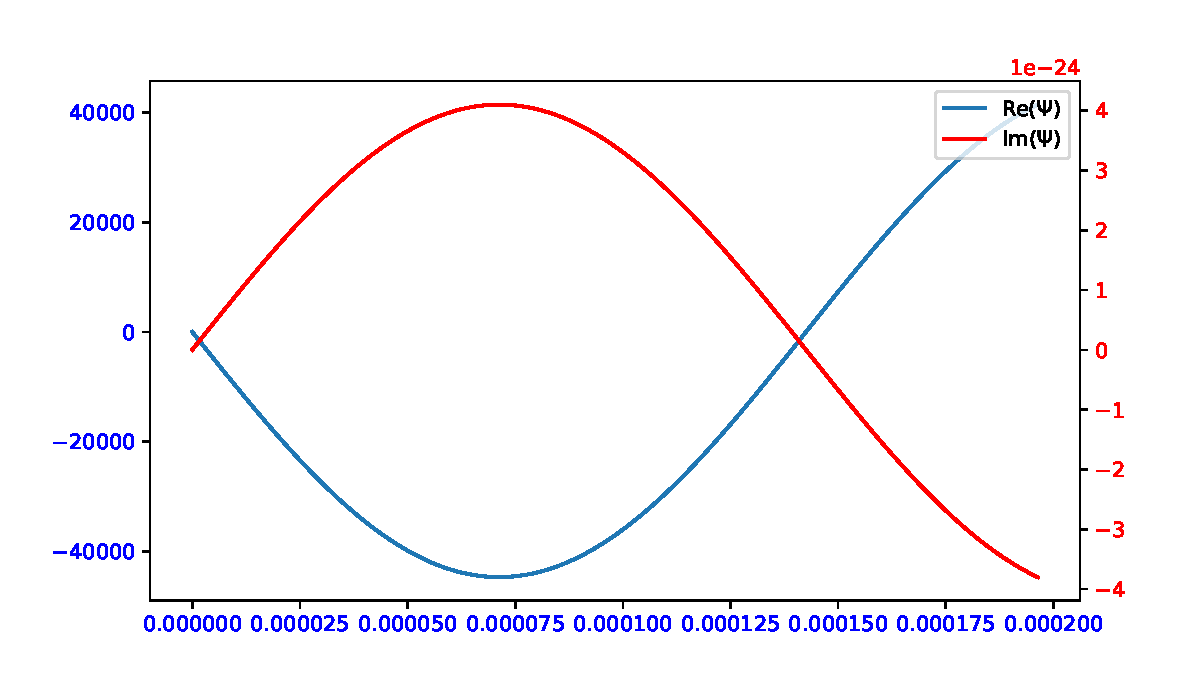
\includegraphics[width = \textwidth]{fig/3.b.1.pdf}
  \caption{Bølgefunksjonen $Ψ$ ved $n = 3$, $a = 1$ nm og $t = 10 fs$. Inkluderer reel og imaginær komponent imaginær}
  \label{fig: 4.b}
\end{figure}
\begin{figure}[h!]
  \centering
  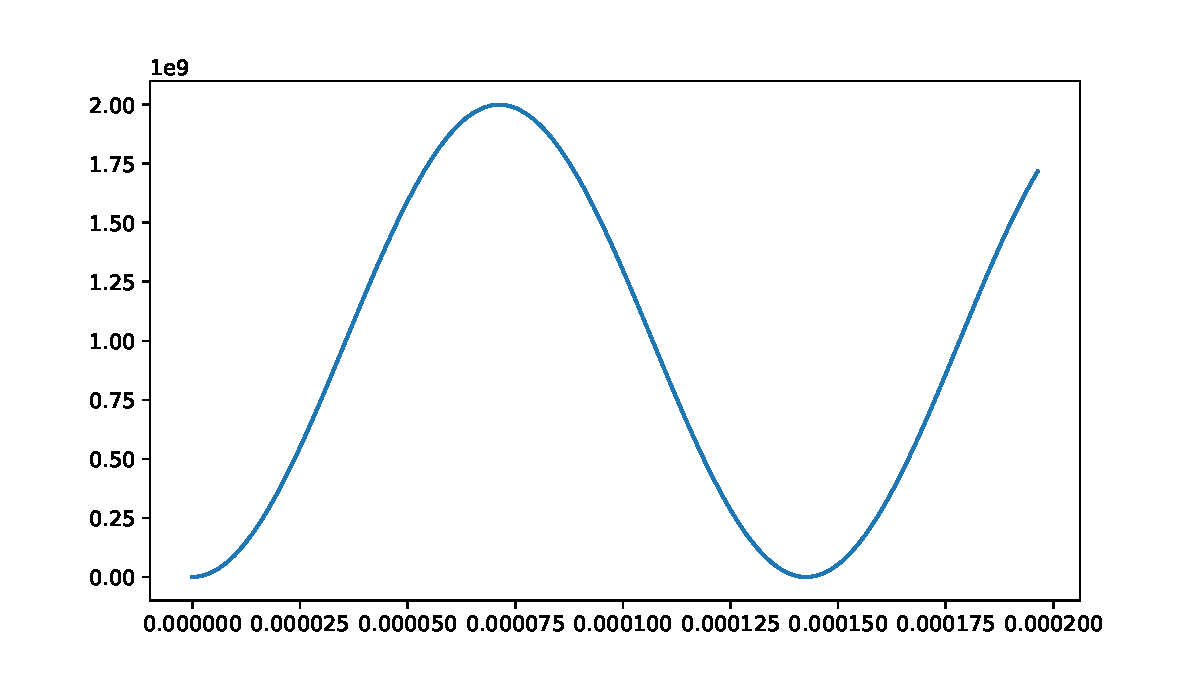
\includegraphics[width = \textwidth]{fig/3.b.2.pdf}
  \caption{Sannsynlighetstettheten for bølgefunksjonen $Ψ$ ved $n = 3$, $a = 1$ nm og $t = 10 fs$.}
  \label{fig: }
\end{figure}
\end{enumerate}

\newpage \phantom{ }
\newpage
\subsection*{Oppgave 4}
\begin{enumerate}[a)]
    \item 
    Vi må løse for forskjellige caser 
    \[
    Ψ(x,0) = 
    \begin{cases}
      A, &\text{ if }0 < x < a / 2\\
      0, &\text{ if }a / 2 < x < a
    \end{cases}
    \]
\end{enumerate}



\end{document}